\documentclass[]{article}
\usepackage{lmodern}
\usepackage{amssymb,amsmath}
\usepackage{ifxetex,ifluatex}
\usepackage{fixltx2e} % provides \textsubscript
\ifnum 0\ifxetex 1\fi\ifluatex 1\fi=0 % if pdftex
  \usepackage[T1]{fontenc}
  \usepackage[utf8]{inputenc}
\else % if luatex or xelatex
  \ifxetex
    \usepackage{mathspec}
  \else
    \usepackage{fontspec}
  \fi
  \defaultfontfeatures{Ligatures=TeX,Scale=MatchLowercase}
\fi
% use upquote if available, for straight quotes in verbatim environments
\IfFileExists{upquote.sty}{\usepackage{upquote}}{}
% use microtype if available
\IfFileExists{microtype.sty}{%
\usepackage{microtype}
\UseMicrotypeSet[protrusion]{basicmath} % disable protrusion for tt fonts
}{}
\usepackage[margin=1in]{geometry}
\usepackage{hyperref}
\hypersetup{unicode=true,
            pdftitle={Exercise 1: Basic Demand Estimation Exercise},
            pdfauthor={Reid Falconer},
            pdfborder={0 0 0},
            breaklinks=true}
\urlstyle{same}  % don't use monospace font for urls
\usepackage{color}
\usepackage{fancyvrb}
\newcommand{\VerbBar}{|}
\newcommand{\VERB}{\Verb[commandchars=\\\{\}]}
\DefineVerbatimEnvironment{Highlighting}{Verbatim}{commandchars=\\\{\}}
% Add ',fontsize=\small' for more characters per line
\usepackage{framed}
\definecolor{shadecolor}{RGB}{248,248,248}
\newenvironment{Shaded}{\begin{snugshade}}{\end{snugshade}}
\newcommand{\AlertTok}[1]{\textcolor[rgb]{0.94,0.16,0.16}{#1}}
\newcommand{\AnnotationTok}[1]{\textcolor[rgb]{0.56,0.35,0.01}{\textbf{\textit{#1}}}}
\newcommand{\AttributeTok}[1]{\textcolor[rgb]{0.77,0.63,0.00}{#1}}
\newcommand{\BaseNTok}[1]{\textcolor[rgb]{0.00,0.00,0.81}{#1}}
\newcommand{\BuiltInTok}[1]{#1}
\newcommand{\CharTok}[1]{\textcolor[rgb]{0.31,0.60,0.02}{#1}}
\newcommand{\CommentTok}[1]{\textcolor[rgb]{0.56,0.35,0.01}{\textit{#1}}}
\newcommand{\CommentVarTok}[1]{\textcolor[rgb]{0.56,0.35,0.01}{\textbf{\textit{#1}}}}
\newcommand{\ConstantTok}[1]{\textcolor[rgb]{0.00,0.00,0.00}{#1}}
\newcommand{\ControlFlowTok}[1]{\textcolor[rgb]{0.13,0.29,0.53}{\textbf{#1}}}
\newcommand{\DataTypeTok}[1]{\textcolor[rgb]{0.13,0.29,0.53}{#1}}
\newcommand{\DecValTok}[1]{\textcolor[rgb]{0.00,0.00,0.81}{#1}}
\newcommand{\DocumentationTok}[1]{\textcolor[rgb]{0.56,0.35,0.01}{\textbf{\textit{#1}}}}
\newcommand{\ErrorTok}[1]{\textcolor[rgb]{0.64,0.00,0.00}{\textbf{#1}}}
\newcommand{\ExtensionTok}[1]{#1}
\newcommand{\FloatTok}[1]{\textcolor[rgb]{0.00,0.00,0.81}{#1}}
\newcommand{\FunctionTok}[1]{\textcolor[rgb]{0.00,0.00,0.00}{#1}}
\newcommand{\ImportTok}[1]{#1}
\newcommand{\InformationTok}[1]{\textcolor[rgb]{0.56,0.35,0.01}{\textbf{\textit{#1}}}}
\newcommand{\KeywordTok}[1]{\textcolor[rgb]{0.13,0.29,0.53}{\textbf{#1}}}
\newcommand{\NormalTok}[1]{#1}
\newcommand{\OperatorTok}[1]{\textcolor[rgb]{0.81,0.36,0.00}{\textbf{#1}}}
\newcommand{\OtherTok}[1]{\textcolor[rgb]{0.56,0.35,0.01}{#1}}
\newcommand{\PreprocessorTok}[1]{\textcolor[rgb]{0.56,0.35,0.01}{\textit{#1}}}
\newcommand{\RegionMarkerTok}[1]{#1}
\newcommand{\SpecialCharTok}[1]{\textcolor[rgb]{0.00,0.00,0.00}{#1}}
\newcommand{\SpecialStringTok}[1]{\textcolor[rgb]{0.31,0.60,0.02}{#1}}
\newcommand{\StringTok}[1]{\textcolor[rgb]{0.31,0.60,0.02}{#1}}
\newcommand{\VariableTok}[1]{\textcolor[rgb]{0.00,0.00,0.00}{#1}}
\newcommand{\VerbatimStringTok}[1]{\textcolor[rgb]{0.31,0.60,0.02}{#1}}
\newcommand{\WarningTok}[1]{\textcolor[rgb]{0.56,0.35,0.01}{\textbf{\textit{#1}}}}
\usepackage{graphicx,grffile}
\makeatletter
\def\maxwidth{\ifdim\Gin@nat@width>\linewidth\linewidth\else\Gin@nat@width\fi}
\def\maxheight{\ifdim\Gin@nat@height>\textheight\textheight\else\Gin@nat@height\fi}
\makeatother
% Scale images if necessary, so that they will not overflow the page
% margins by default, and it is still possible to overwrite the defaults
% using explicit options in \includegraphics[width, height, ...]{}
\setkeys{Gin}{width=\maxwidth,height=\maxheight,keepaspectratio}
\IfFileExists{parskip.sty}{%
\usepackage{parskip}
}{% else
\setlength{\parindent}{0pt}
\setlength{\parskip}{6pt plus 2pt minus 1pt}
}
\setlength{\emergencystretch}{3em}  % prevent overfull lines
\providecommand{\tightlist}{%
  \setlength{\itemsep}{0pt}\setlength{\parskip}{0pt}}
\setcounter{secnumdepth}{0}
% Redefines (sub)paragraphs to behave more like sections
\ifx\paragraph\undefined\else
\let\oldparagraph\paragraph
\renewcommand{\paragraph}[1]{\oldparagraph{#1}\mbox{}}
\fi
\ifx\subparagraph\undefined\else
\let\oldsubparagraph\subparagraph
\renewcommand{\subparagraph}[1]{\oldsubparagraph{#1}\mbox{}}
\fi

%%% Use protect on footnotes to avoid problems with footnotes in titles
\let\rmarkdownfootnote\footnote%
\def\footnote{\protect\rmarkdownfootnote}

%%% Change title format to be more compact
\usepackage{titling}

% Create subtitle command for use in maketitle
\newcommand{\subtitle}[1]{
  \posttitle{
    \begin{center}\large#1\end{center}
    }
}

\setlength{\droptitle}{-2em}

  \title{Exercise 1: Basic Demand Estimation Exercise}
    \pretitle{\vspace{\droptitle}\centering\huge}
  \posttitle{\par}
    \author{Reid Falconer}
    \preauthor{\centering\large\emph}
  \postauthor{\par}
      \predate{\centering\large\emph}
  \postdate{\par}
    \date{2018-10-14}


\begin{document}
\maketitle

\leavevmode\hypertarget{logo-container}{}%

\hypertarget{data-check}{%
\subsection{Data Check}\label{data-check}}

\hypertarget{construct-a-price-variable-by-dividing-sales-by-unit-sales-employ-the-sales_-and-sales_u-variables.-explain-how-to-interpret-this-price-variable-i.e.what-sort-of-average-price-is-this.}{%
\subparagraph{\texorpdfstring{1. Construct a price variable by dividing
\$ sales by unit sales (employ the \texttt{sales\_\$} and
\texttt{sales\_u} variables). Explain how to interpret this price
variable (i.e.~what sort of average price is
this?).}{1. Construct a price variable by dividing \$ sales by unit sales (employ the sales\_\$ and sales\_u variables). Explain how to interpret this price variable (i.e.~what sort of average price is this?).}}\label{construct-a-price-variable-by-dividing-sales-by-unit-sales-employ-the-sales_-and-sales_u-variables.-explain-how-to-interpret-this-price-variable-i.e.what-sort-of-average-price-is-this.}}

\begin{Shaded}
\begin{Highlighting}[]
\NormalTok{price <-}\StringTok{ }\NormalTok{mydata}\OperatorTok{$}\NormalTok{Sales_USD}\OperatorTok{/}\NormalTok{mydata}\OperatorTok{$}\NormalTok{Sales_U  }\CommentTok{# See `createVariables` function in `ex1hints.R`. }
\end{Highlighting}
\end{Shaded}

The constructed `price' varible is the average price of one unit
(equivalent units (lbs)) of the item in USD(\$).

\hypertarget{compute-the-mean-prices-across-weeks-of-hellmans-in-jewel-and-the-central-region.-are-they-comparable-repeat-the-exercise-for-kraft-in-jewel-and-the-central-region.}{%
\subparagraph{2. Compute the mean prices across weeks of Hellman's in
Jewel and the Central Region. Are they comparable? Repeat the exercise
for Kraft in Jewel and the Central
Region.}\label{compute-the-mean-prices-across-weeks-of-hellmans-in-jewel-and-the-central-region.-are-they-comparable-repeat-the-exercise-for-kraft-in-jewel-and-the-central-region.}}

\hypertarget{hellmans}{%
\paragraph{Hellmans}\label{hellmans}}

\begin{Shaded}
\begin{Highlighting}[]
\NormalTok{df_hellman <-}\StringTok{ }\KeywordTok{na.omit}\NormalTok{(}\KeywordTok{cbind}\NormalTok{(hellman_at_jewel}\OperatorTok{$}\NormalTok{price, hellman_at_central}\OperatorTok{$}\NormalTok{price)) }\OperatorTok\StringTok{ }
\StringTok{  }\KeywordTok{as.data.frame}\NormalTok{() }\OperatorTok\StringTok{ }
\StringTok{  }\KeywordTok{rename}\NormalTok{(}\DataTypeTok{hellman_at_jewel_price =}\NormalTok{ V1,}
         \DataTypeTok{hellman_at_central_price =}\NormalTok{ V2) }\OperatorTok\StringTok{ }
\StringTok{  }\KeywordTok{gather}\NormalTok{(region, value)}

\NormalTok{mu_hellman <-}\StringTok{ }\NormalTok{df_hellman }\OperatorTok\StringTok{ }\KeywordTok{group_by}\NormalTok{(region) }\OperatorTok\StringTok{ }\KeywordTok{summarize}\NormalTok{(}\DataTypeTok{grp_mean =} \KeywordTok{mean}\NormalTok{(value))}

\NormalTok{t_test_hellman <-}\StringTok{ }\KeywordTok{t.test}\NormalTok{(value }\OperatorTok{~}\StringTok{ }\NormalTok{region, }\DataTypeTok{data =}\NormalTok{ df_hellman)}
\end{Highlighting}
\end{Shaded}

\begin{center}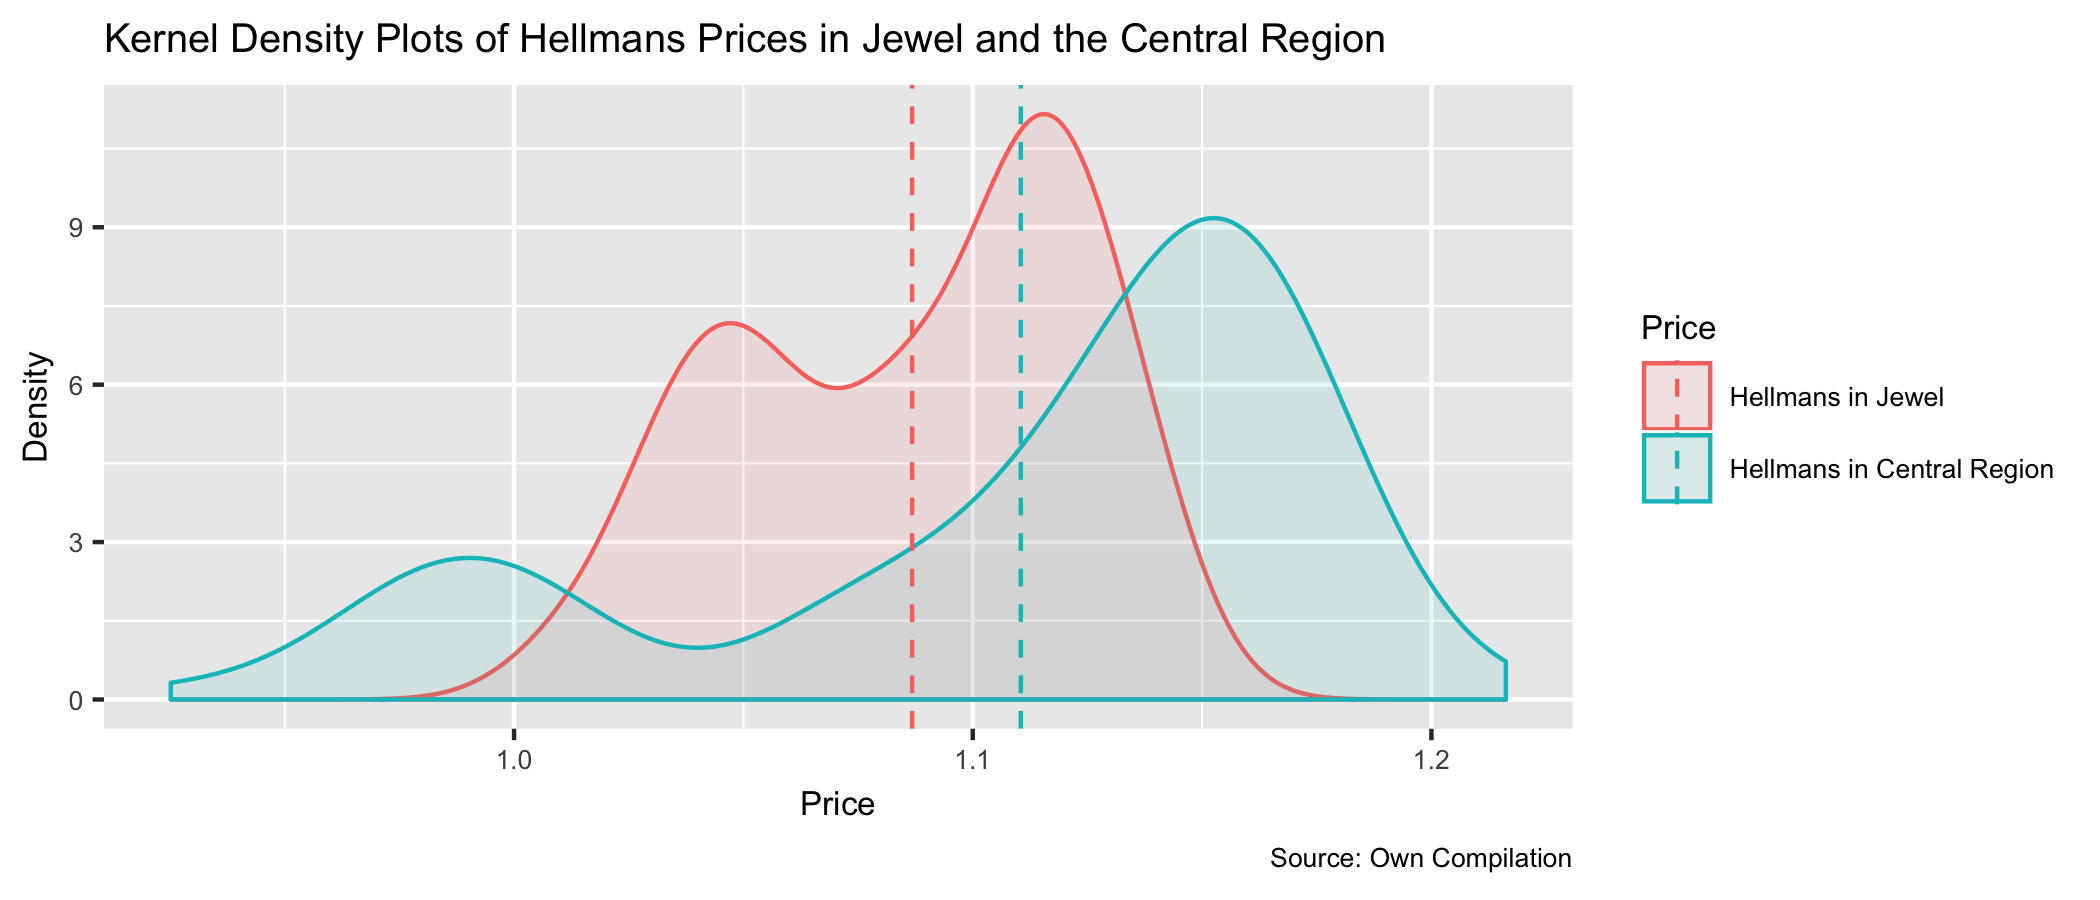
\includegraphics{Exercise_1_print_files/figure-latex/unnamed-chunk-3-1} \end{center}

The mean price of Hellman's in the Jewel Region is \$1.11 while the mean
price of Hellman's in the Central Region is \$1.087. These prices seem
comparable. However, after conducting a two-tailed t-test one finds that
the means are significantly different at a approximaly a 2\% level of
significance (p-value =0.002).

\hypertarget{kraft}{%
\paragraph{Kraft}\label{kraft}}

\begin{Shaded}
\begin{Highlighting}[]
\NormalTok{df_kraft <-}\StringTok{ }\KeywordTok{na.omit}\NormalTok{(}\KeywordTok{cbind}\NormalTok{(kraft_at_jewel}\OperatorTok{$}\NormalTok{price, kraft_at_central}\OperatorTok{$}\NormalTok{price)) }\OperatorTok\StringTok{ }
\StringTok{  }\KeywordTok{as.data.frame}\NormalTok{() }\OperatorTok\StringTok{ }
\StringTok{  }\KeywordTok{rename}\NormalTok{(}\DataTypeTok{kraft_at_jewel_price =}\NormalTok{ V1,}
         \DataTypeTok{kraft_at_central_price =}\NormalTok{ V2) }\OperatorTok\StringTok{ }
\StringTok{  }\KeywordTok{gather}\NormalTok{(region, value)}

\NormalTok{mu_kraft <-}\StringTok{ }\NormalTok{df_kraft }\OperatorTok\StringTok{ }\KeywordTok{group_by}\NormalTok{(region) }\OperatorTok\StringTok{ }\KeywordTok{summarize}\NormalTok{(}\DataTypeTok{grp_mean =} \KeywordTok{mean}\NormalTok{(value))}

\NormalTok{t_test_kraft <-}\StringTok{ }\KeywordTok{t.test}\NormalTok{(value }\OperatorTok{~}\StringTok{ }\NormalTok{region, }\DataTypeTok{data =}\NormalTok{ df_kraft)}
\end{Highlighting}
\end{Shaded}

\begin{center}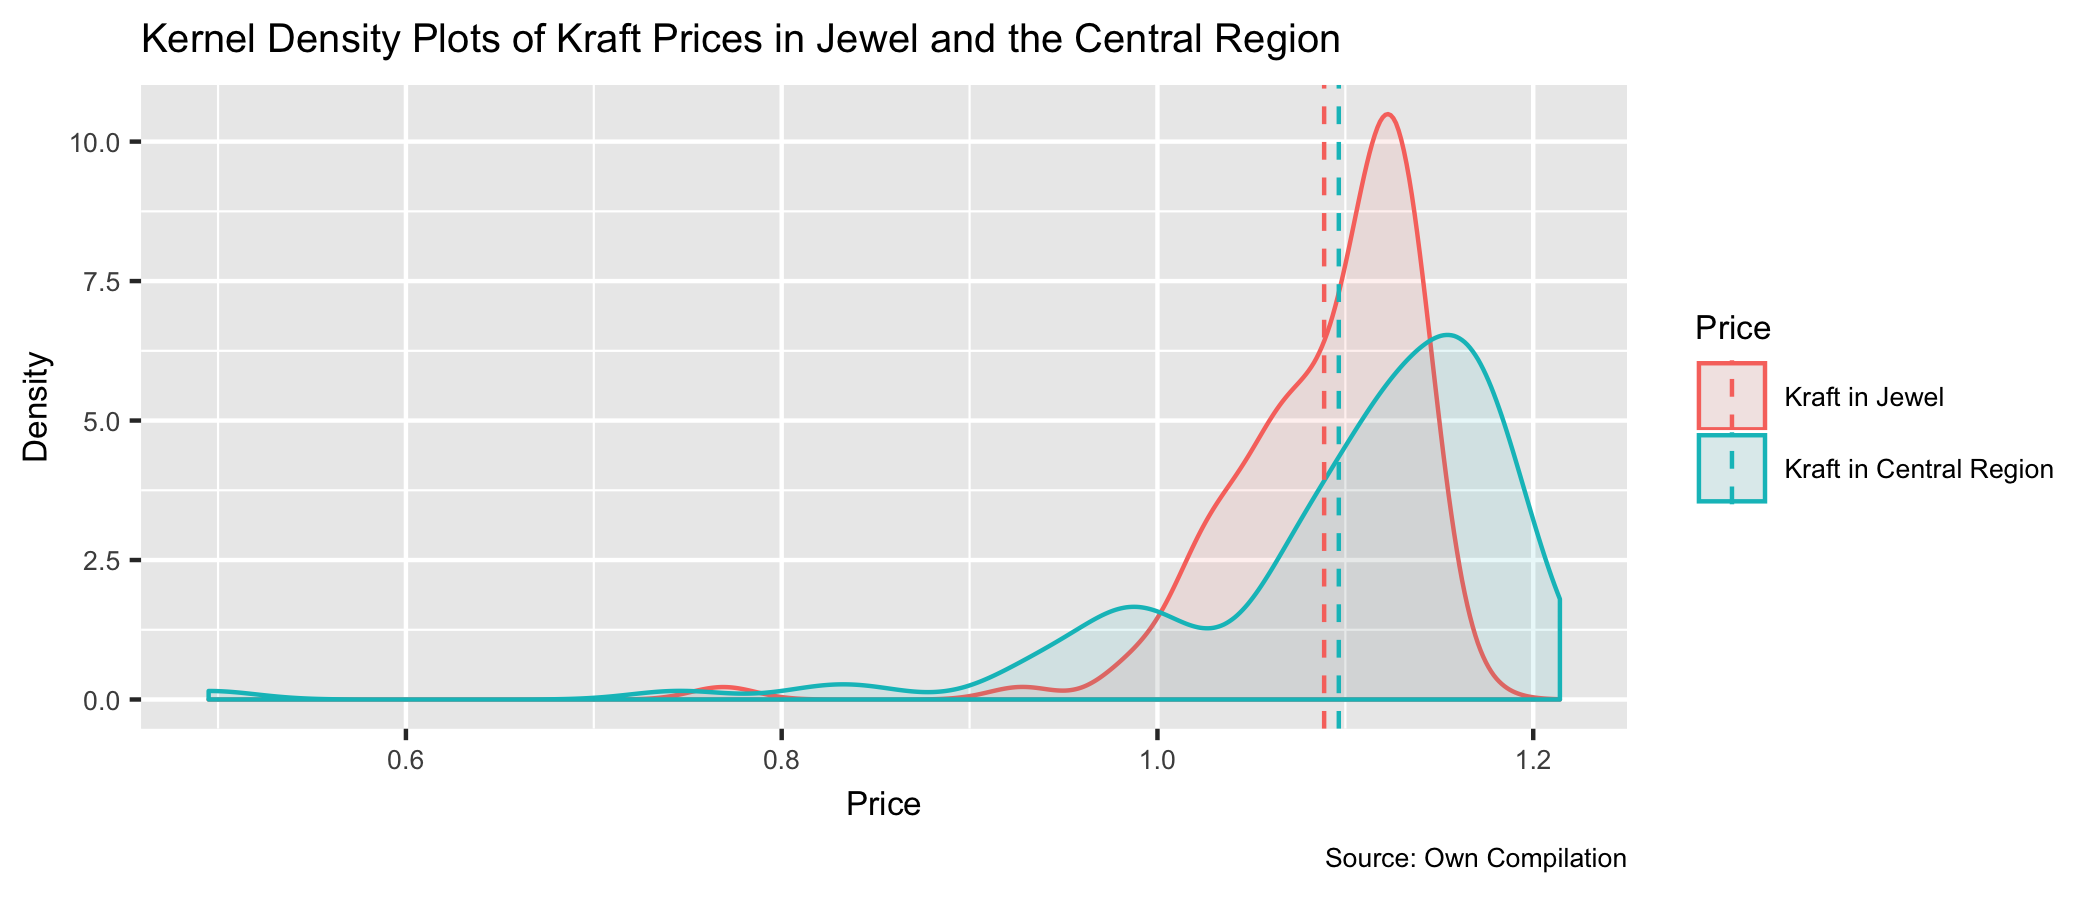
\includegraphics{Exercise_1_print_files/figure-latex/unnamed-chunk-5-1} \end{center}

The mean price of Kraft in the Jewel Region is \$1.097 while the mean
price of Kraft in the Central Region is \$1.089. These prices are
comparable and after conducting a two-tailed t-test one finds that the
means are not significantly different from one another (p-value =0.002).

\hypertarget{price-variation-compute-the-standard-deviation-of-prices-across-weeks-of-hellmans-in-jewel-and-the-central-region.-is-there-more-price-variation-at-jewel-or-in-the-central-region-why-what-does-this-tell-you-upfront-about-your-ability-to-estimate-price-elasticities-with-either-account-level-data-or-data-in-a-large-geographic-market-repeat-the-exercise-for-kraft-in-jewel-and-the-central-region.}{%
\subparagraph{3. Price variation: Compute the standard deviation of
prices across weeks of Hellman's in Jewel and the Central Region. Is
there more price variation at Jewel or in the Central Region? Why? What
does this tell you upfront about your ability to estimate price
elasticities with either account level data or data in a large
geographic market? Repeat the exercise for Kraft in Jewel and the
Central
Region.}\label{price-variation-compute-the-standard-deviation-of-prices-across-weeks-of-hellmans-in-jewel-and-the-central-region.-is-there-more-price-variation-at-jewel-or-in-the-central-region-why-what-does-this-tell-you-upfront-about-your-ability-to-estimate-price-elasticities-with-either-account-level-data-or-data-in-a-large-geographic-market-repeat-the-exercise-for-kraft-in-jewel-and-the-central-region.}}

\begin{Shaded}
\begin{Highlighting}[]
\NormalTok{sd_hellman <-}\StringTok{ }\NormalTok{df_hellman }\OperatorTok\StringTok{ }\KeywordTok{group_by}\NormalTok{(region) }\OperatorTok\StringTok{ }\KeywordTok{summarize}\NormalTok{(}\DataTypeTok{grp_sd =} \KeywordTok{sd}\NormalTok{(value))}
\NormalTok{sd_kraft <-}\StringTok{ }\NormalTok{df_kraft }\OperatorTok\StringTok{ }\KeywordTok{group_by}\NormalTok{(region) }\OperatorTok\StringTok{ }\KeywordTok{summarize}\NormalTok{(}\DataTypeTok{grp_sd =} \KeywordTok{sd}\NormalTok{(value))}
\end{Highlighting}
\end{Shaded}

The standard deviation for Hellman's in the Jewel region is noticeably
greater than in the Central region. (0.068 vs 0.037 standard deviation
respectivly). Similarily, the standard deviation for Kraft in the Jewel
region is significantly larger than in the Central region. (0.105 and
0.054 standard deviation respectivly)

What does this tell you upfront about your ability to estimate price
elasticities?

\hypertarget{price-plots-construct-time-series-plots-of-sales-and-prices-for-hellmans-in-the-central-division-and-for-jewel-i.e.weeks-on-the-x-axis-prices-and-unit-sales-on-the-y-axis.-repeat-the-exercise-for-kraft.-describe-the-differences-or-similarities-between-kraft-and-hellmans-pricing-policies-in-each-account.}{%
\subparagraph{4. Price plots: Construct time-series plots of sales and
prices for Hellmans in the Central division and for Jewel (i.e.~weeks on
the X-axis, prices and unit-sales on the Y-axis). Repeat the exercise
for Kraft. Describe the differences or similarities between Kraft and
Hellman's pricing policies in each
account.}\label{price-plots-construct-time-series-plots-of-sales-and-prices-for-hellmans-in-the-central-division-and-for-jewel-i.e.weeks-on-the-x-axis-prices-and-unit-sales-on-the-y-axis.-repeat-the-exercise-for-kraft.-describe-the-differences-or-similarities-between-kraft-and-hellmans-pricing-policies-in-each-account.}}

\hypertarget{hellmans-1}{%
\paragraph{Hellmans}\label{hellmans-1}}

\begin{center}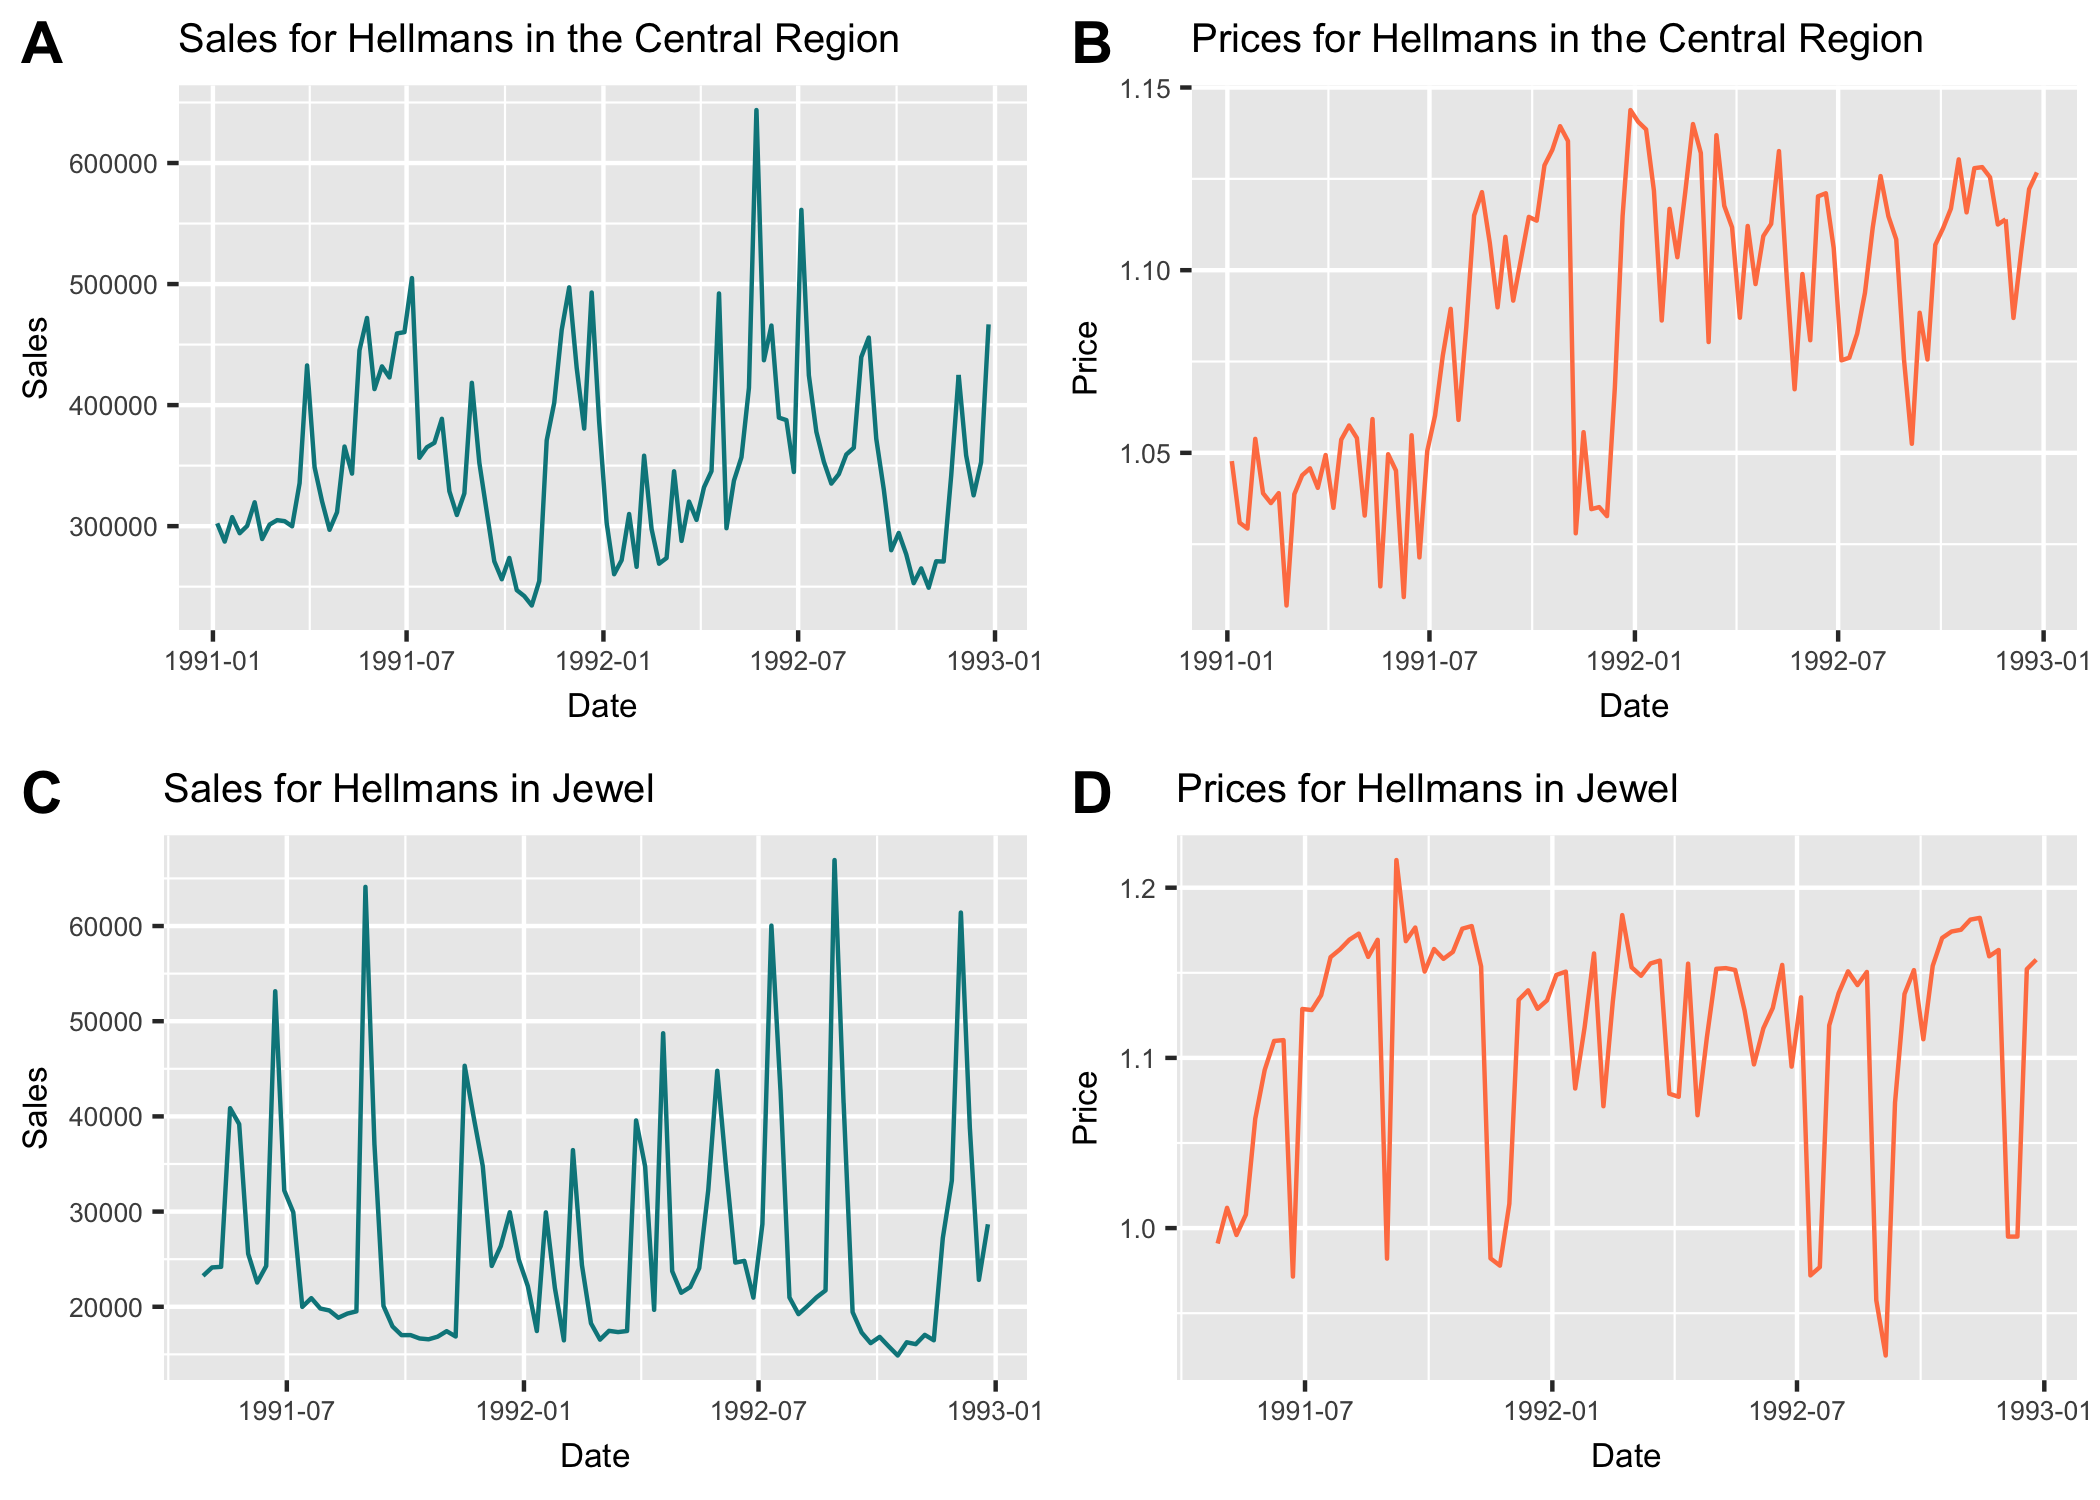
\includegraphics{Exercise_1_print_files/figure-latex/unnamed-chunk-7-1} \end{center}

\hypertarget{kraft-1}{%
\paragraph{Kraft}\label{kraft-1}}

\begin{center}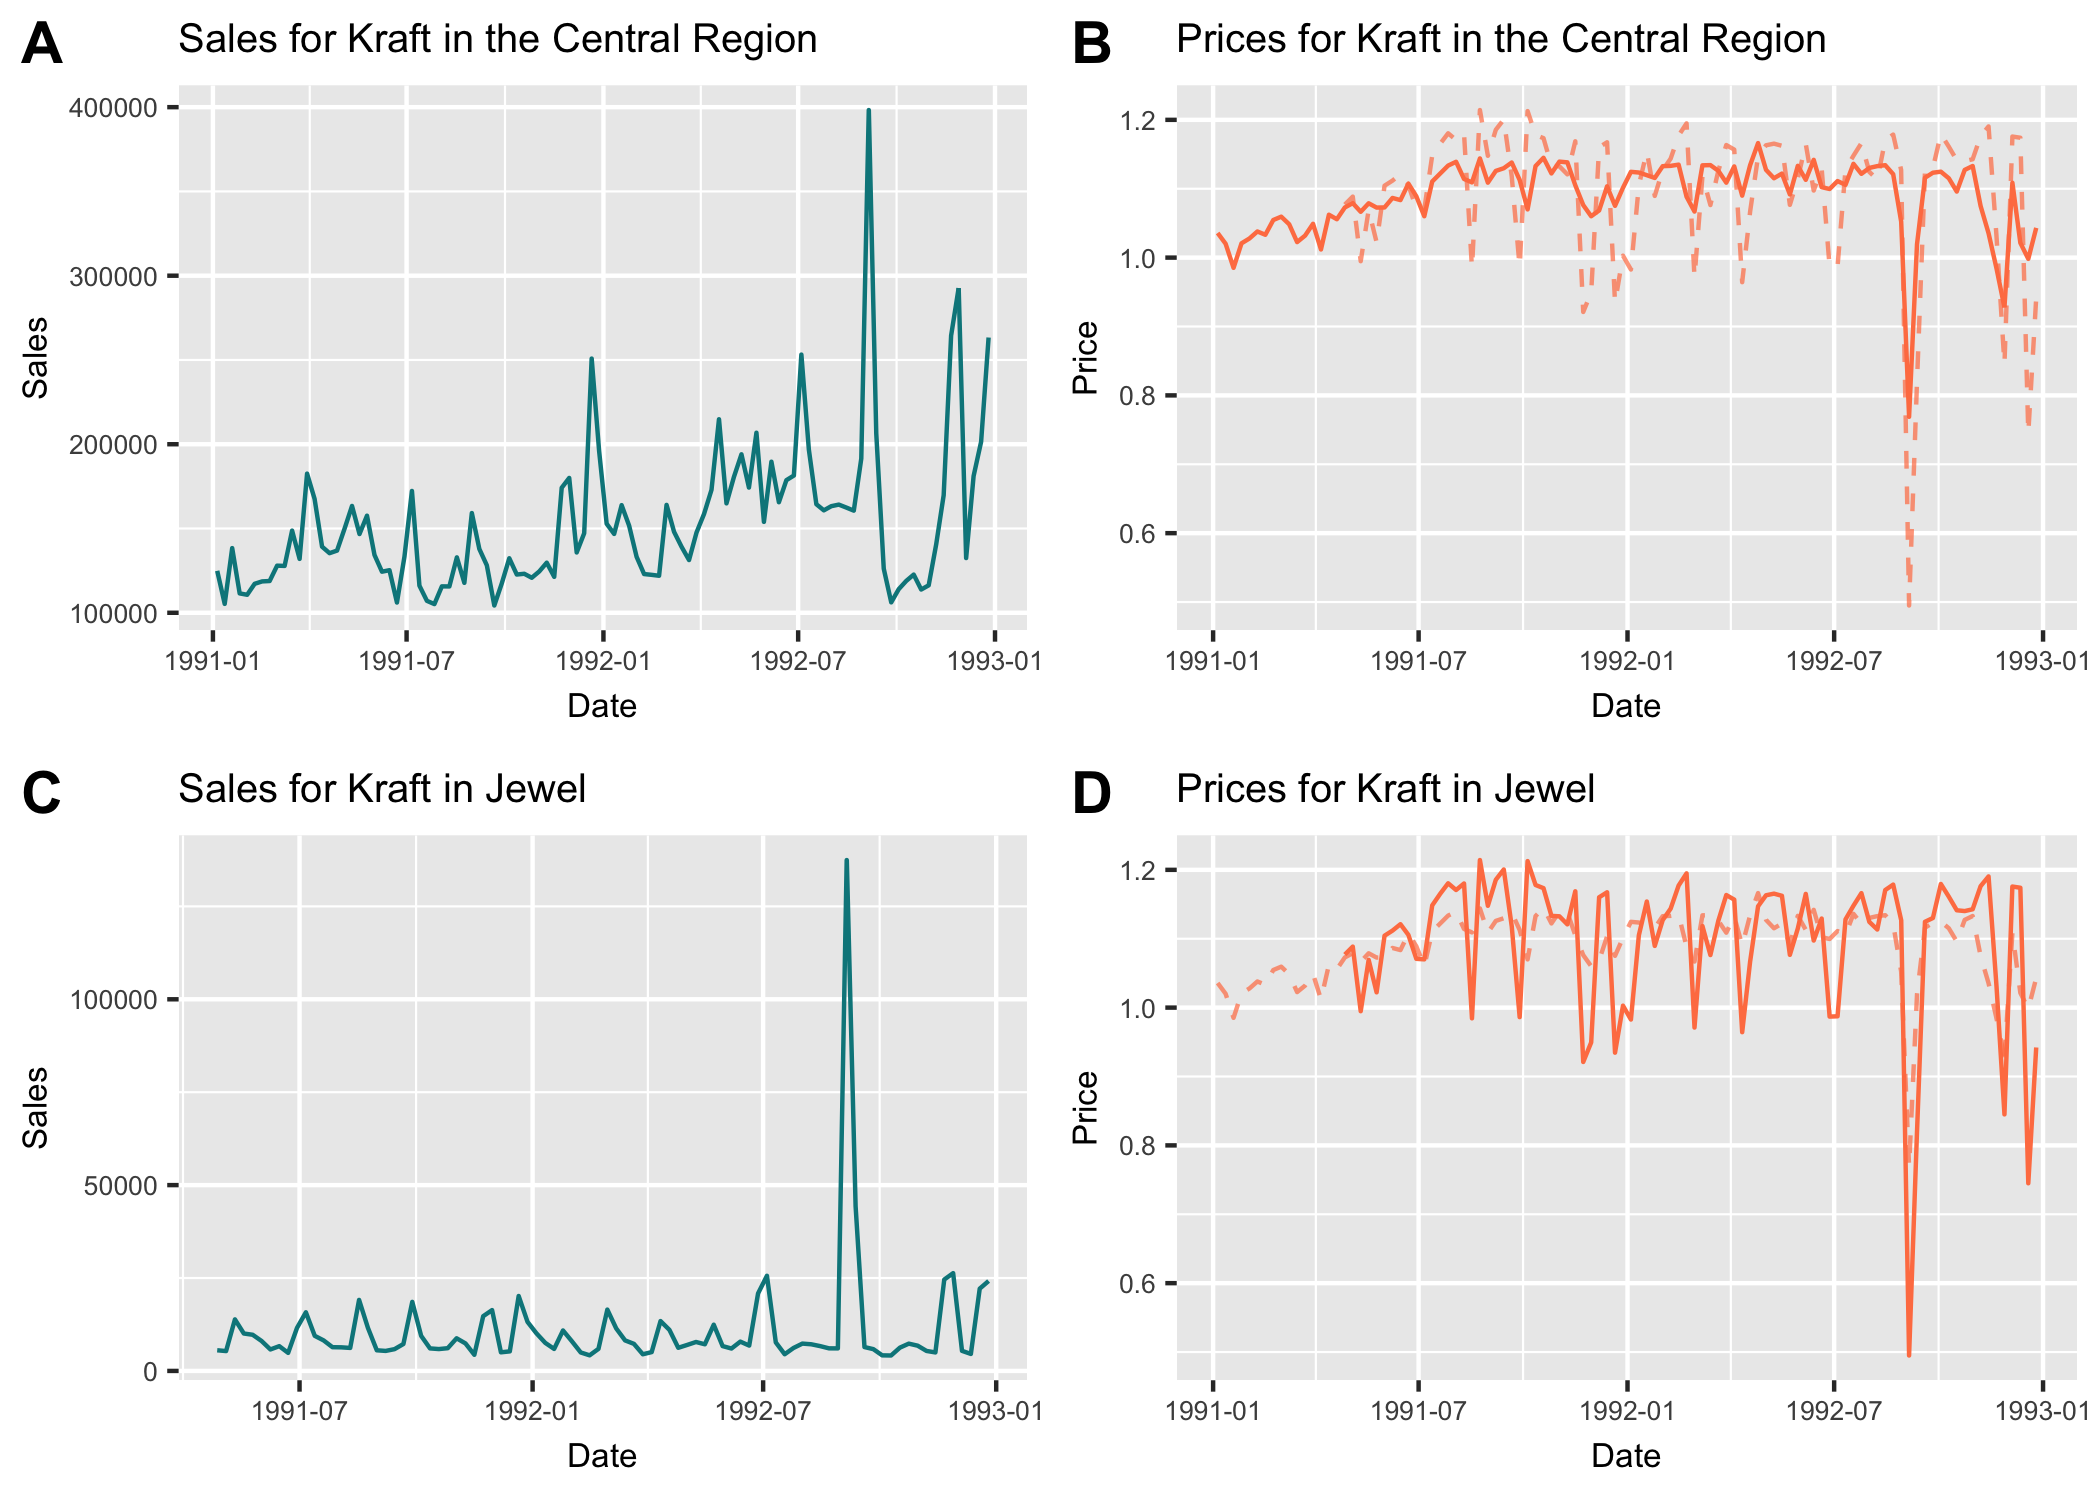
\includegraphics{Exercise_1_print_files/figure-latex/unnamed-chunk-8-1} \end{center}

\hypertarget{scatter-plots-construct-scatter-plots-of-sales-versus-prices-for-hellmans-in-the-central-division-and-for-jewel-i.e.prices-on-the-y-axis-unit-sales-on-the-x-axis.-repeat-the-exercise-for-kraft.-is-there-evidence-for-a-negatively-sloped-demand-curve-in-the-data-eye-balling-these-plots-does-demand-appear-more-elastic-in-the-central-region-or-at-jewel-for-either-hellmans-or-kraft}{%
\subparagraph{5. Scatter-plots: Construct scatter-plots of sales versus
prices for Hellmans in the Central division and for Jewel (i.e.~prices
on the Y-axis, unit-sales on the X-axis). Repeat the exercise for Kraft.
Is there evidence for a negatively sloped demand-curve in the data?
Eye-balling these plots, does demand appear more elastic in the Central
Region or at Jewel (for either Hellman's or
Kraft)?}\label{scatter-plots-construct-scatter-plots-of-sales-versus-prices-for-hellmans-in-the-central-division-and-for-jewel-i.e.prices-on-the-y-axis-unit-sales-on-the-x-axis.-repeat-the-exercise-for-kraft.-is-there-evidence-for-a-negatively-sloped-demand-curve-in-the-data-eye-balling-these-plots-does-demand-appear-more-elastic-in-the-central-region-or-at-jewel-for-either-hellmans-or-kraft}}

\hypertarget{hellmans-2}{%
\paragraph{Hellmans}\label{hellmans-2}}

\begin{center}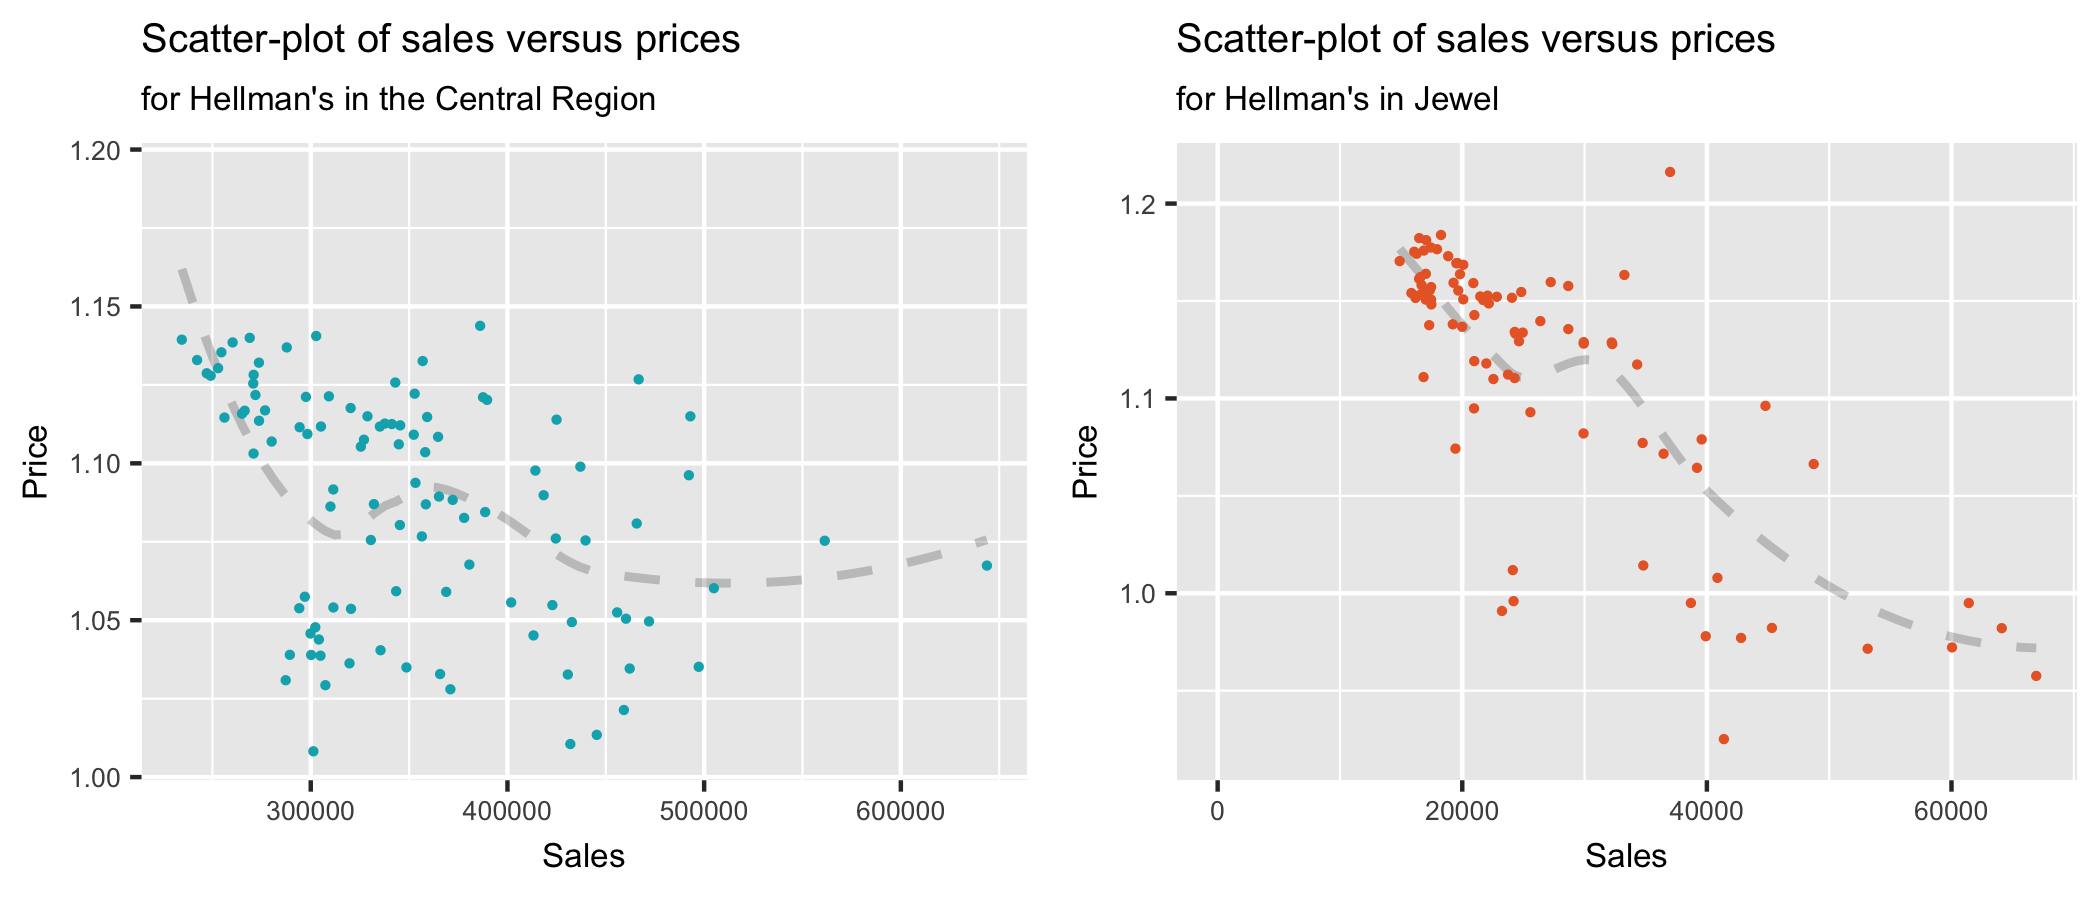
\includegraphics{Exercise_1_print_files/figure-latex/unnamed-chunk-9-1} \end{center}

\hypertarget{kraft-2}{%
\paragraph{Kraft}\label{kraft-2}}

\begin{center}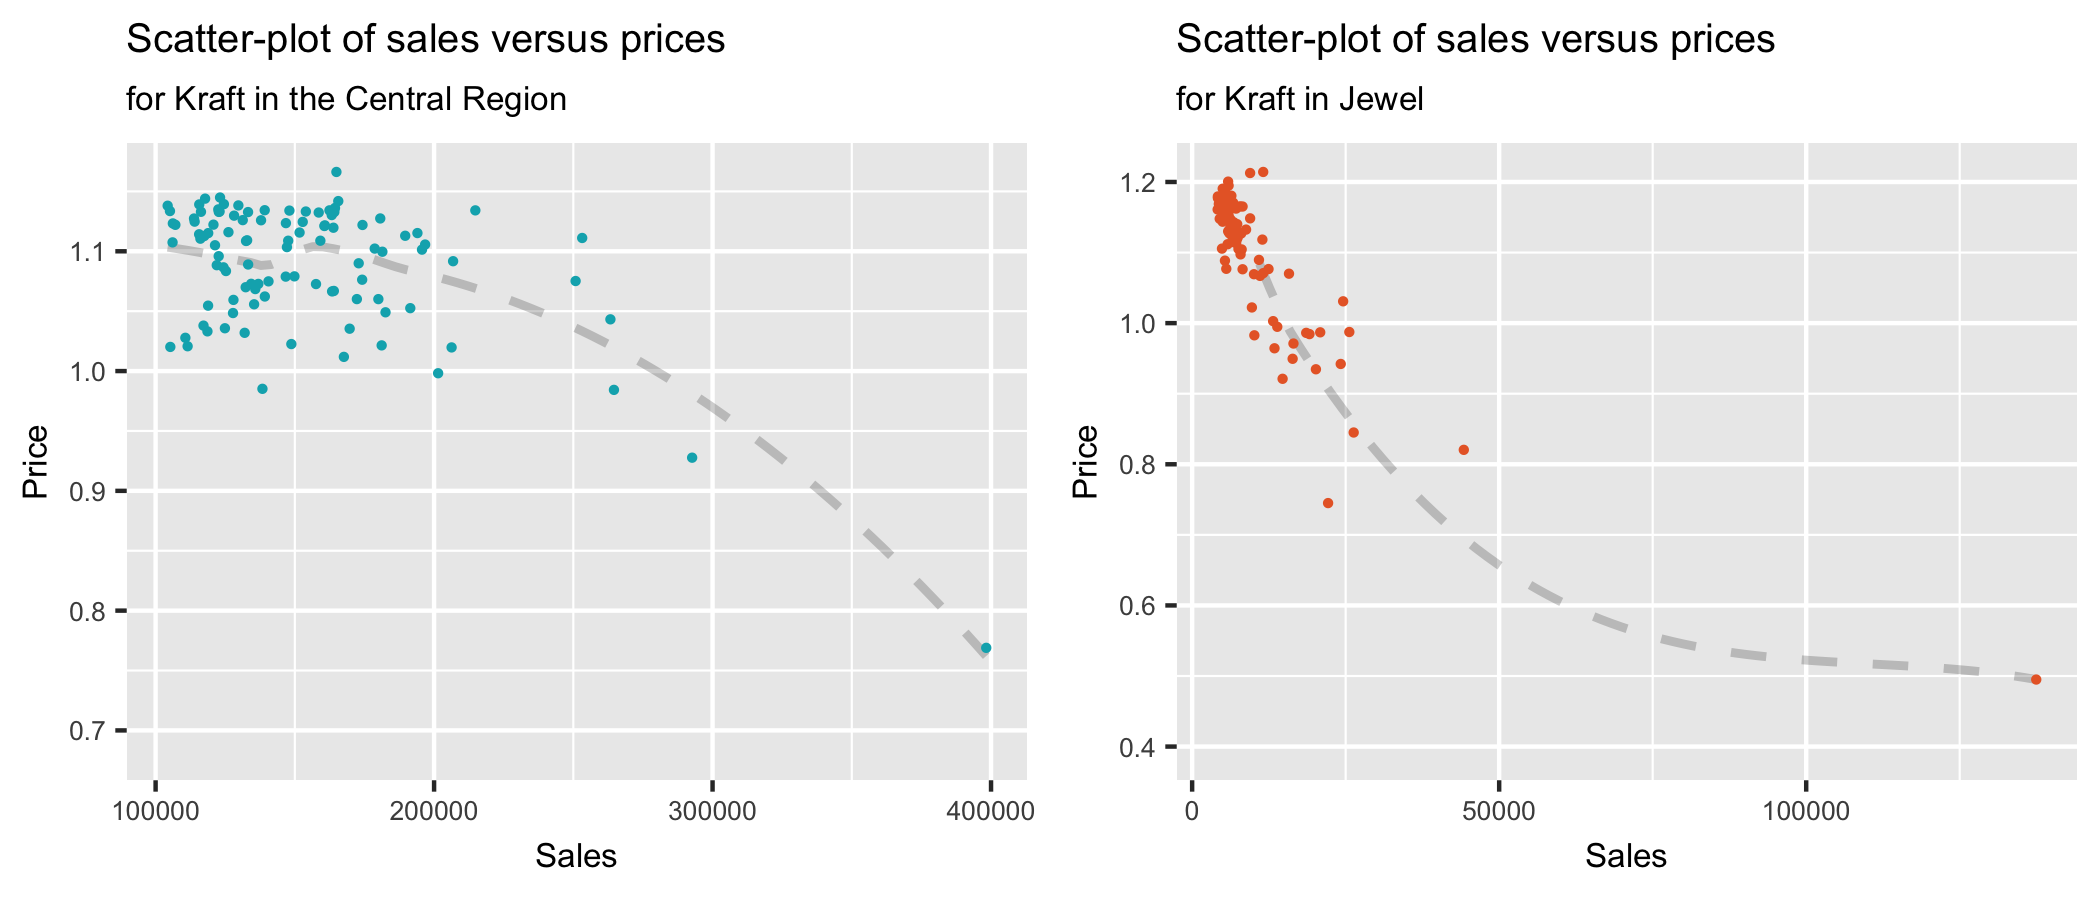
\includegraphics{Exercise_1_print_files/figure-latex/unnamed-chunk-10-1} \end{center}

\hypertarget{demand-estimation}{%
\subsection{Demand Estimation}\label{demand-estimation}}

\hypertarget{fit-the-multiplicative-demand-model-discussed-in-class-for-kraft-and-hellmans-at-jewel-i.e.2-separate-regressions-one-for-hellmans-and-one-for-kraft.}{%
\subparagraph{1. Fit the ``multiplicative'' demand model discussed in
class for Kraft and Hellman's at Jewel (i.e.~2 separate regressions, one
for Hellman's, and one for
Kraft).}\label{fit-the-multiplicative-demand-model-discussed-in-class-for-kraft-and-hellmans-at-jewel-i.e.2-separate-regressions-one-for-hellmans-and-one-for-kraft.}}

\hypertarget{hellman-at-jewel}{%
\paragraph{Hellman at Jewel}\label{hellman-at-jewel}}

\begin{Shaded}
\begin{Highlighting}[]
\NormalTok{model_}\DecValTok{1}\NormalTok{ <-}\StringTok{ }\KeywordTok{runRegression}\NormalTok{(hellman_at_jewel)}
\end{Highlighting}
\end{Shaded}

Sales of Hellman at Jewel

ln(Hellman Sales)

OLS

ln(Hellman price)

-4.580***

(0.427)

Constant

10.600***

(0.053)

Observations

88

R2

0.573

Adjusted R2

0.568

Residual Std. Error

0.248 (df = 86)

F Statistic

115.000*** (df = 1; 86)

Note:

\emph{p\textless{}0.1; \textbf{p\textless{}0.05; }}p\textless{}0.01

\hypertarget{kraft-at-jewel}{%
\paragraph{Kraft at Jewel}\label{kraft-at-jewel}}

\begin{Shaded}
\begin{Highlighting}[]
\NormalTok{model_}\DecValTok{2}\NormalTok{ <-}\StringTok{ }\KeywordTok{runRegression}\NormalTok{(kraft_at_jewel)}
\end{Highlighting}
\end{Shaded}

Sales of Kraft at Jewel

ln(Kraft Sales)

OLS

ln(Kraft price)

-4.170***

(0.254)

Constant

9.400***

(0.038)

Observations

88

R2

0.758

Adjusted R2

0.756

Residual Std. Error

0.292 (df = 86)

F Statistic

270.000*** (df = 1; 86)

Note:

\emph{p\textless{}0.1; \textbf{p\textless{}0.05; }}p\textless{}0.01

\hypertarget{fit-the-multiplicative-demand-model-discussed-in-class-for-kraft-and-hellmans-for-the-central-region-i.e.2-separate-regressions-one-for-hellmans-and-one-for-kraft.}{%
\subparagraph{2. Fit the ``multiplicative'' demand model discussed in
class for Kraft and Hellman's for the Central Region (i.e.~2 separate
regressions, one for Hellman's, and one for
Kraft).}\label{fit-the-multiplicative-demand-model-discussed-in-class-for-kraft-and-hellmans-for-the-central-region-i.e.2-separate-regressions-one-for-hellmans-and-one-for-kraft.}}

\hypertarget{hellman-at-central}{%
\paragraph{Hellman at Central}\label{hellman-at-central}}

\begin{Shaded}
\begin{Highlighting}[]
\NormalTok{model_}\DecValTok{3}\NormalTok{ <-}\StringTok{ }\KeywordTok{runRegression}\NormalTok{(hellman_at_central)}
\end{Highlighting}
\end{Shaded}

Sales of Hellman at Central

ln(Hellman Sales)

OLS

ln(Hellman price)

-2.380***

(0.551)

Constant

12.900***

(0.049)

Observations

104

R2

0.154

Adjusted R2

0.146

Residual Std. Error

0.190 (df = 102)

F Statistic

18.600*** (df = 1; 102)

Note:

\emph{p\textless{}0.1; \textbf{p\textless{}0.05; }}p\textless{}0.01

\hypertarget{kraft-at-central}{%
\paragraph{Kraft at Central}\label{kraft-at-central}}

\begin{Shaded}
\begin{Highlighting}[]
\NormalTok{model_}\DecValTok{4}\NormalTok{ <-}\StringTok{ }\KeywordTok{runRegression}\NormalTok{(kraft_at_central)}
\end{Highlighting}
\end{Shaded}

Sales of Kraft at Central

ln(Kraft Sales)

OLS

ln(Kraft price)

-2.110***

(0.401)

Constant

12.100***

(0.040)

Observations

104

R2

0.213

Adjusted R2

0.205

Residual Std. Error

0.218 (df = 102)

F Statistic

27.600*** (df = 1; 102)

Note:

\emph{p\textless{}0.1; \textbf{p\textless{}0.05; }}p\textless{}0.01

\hypertarget{elasticity-differences-is-the-demand-elasticity-higher-in-absolute-magnitude-at-the-jewel-account-or-in-the-central-region-can-you-offer-some-compelling-explanations-for-the-difference-think-of-as-many-potential-reasons-as-possible}{%
\subparagraph{3. Elasticity differences: Is the demand elasticity higher
(in absolute magnitude) at the Jewel account or in the Central Region?
Can you offer some compelling explanations for the difference? (think of
as many potential reasons as
possible)}\label{elasticity-differences-is-the-demand-elasticity-higher-in-absolute-magnitude-at-the-jewel-account-or-in-the-central-region-can-you-offer-some-compelling-explanations-for-the-difference-think-of-as-many-potential-reasons-as-possible}}

\hypertarget{forecasting-demand-under-a-price-change-using-your-regression-results-from-the-multiplicative-demand-model-compute-the-change-in-unit-sales-for-a-10-increase-in-the-price-of-kraft-and-hellmans-at-jewel.-note-you-can-do-this-brute-force-in-excel-but-for-your-benefit-you-should-try-to-compute-this-on-a-sheet-of-paper-with-the-help-of-a-calculator.}{%
\subparagraph{4. Forecasting demand under a price change: Using your
regression results from the multiplicative demand model, compute the \%
change in unit sales for a 10\% increase in the price of Kraft and
Hellman's at Jewel. (Note: You can do this brute force in Excel, but for
your benefit you should try to compute this on a sheet of paper with the
help of a
calculator).}\label{forecasting-demand-under-a-price-change-using-your-regression-results-from-the-multiplicative-demand-model-compute-the-change-in-unit-sales-for-a-10-increase-in-the-price-of-kraft-and-hellmans-at-jewel.-note-you-can-do-this-brute-force-in-excel-but-for-your-benefit-you-should-try-to-compute-this-on-a-sheet-of-paper-with-the-help-of-a-calculator.}}

\hypertarget{hellman-at-jewel-1}{%
\paragraph{Hellman at Jewel}\label{hellman-at-jewel-1}}

\begin{Shaded}
\begin{Highlighting}[]
\CommentTok{# To get the proportional change in Y associated with a p percent increase in X, calculate}
\CommentTok{# a = ([100 + p]/100) and take a^β}
\NormalTok{price_coeff <-}\StringTok{ }\NormalTok{tidy_model_}\DecValTok{1}\OperatorTok{$}\NormalTok{estimate[}\DecValTok{2}\NormalTok{]}

\NormalTok{compute_change <-}\StringTok{ }\ControlFlowTok{function}\NormalTok{(percent_change, price_coeff) \{}
\NormalTok{  a <-}\StringTok{ }\NormalTok{((}\DecValTok{100} \OperatorTok{+}\StringTok{ }\NormalTok{percent_change)}\OperatorTok{/}\DecValTok{100}\NormalTok{)}
\NormalTok{  price_effect <-}\StringTok{ }\NormalTok{a}\OperatorTok{^}\NormalTok{price_coeff}
  \ControlFlowTok{if}\NormalTok{ (price_effect }\OperatorTok{<}\StringTok{ }\DecValTok{1}\NormalTok{) \{}
\NormalTok{  prop <-}\StringTok{ }\KeywordTok{round}\NormalTok{((}\DecValTok{1}\OperatorTok{-}\NormalTok{price_effect)}\OperatorTok{*}\DecValTok{100}\NormalTok{, }\DataTypeTok{digits =} \DecValTok{2}\NormalTok{)}
\NormalTok{  direction <-}\StringTok{ "% decrease"}
\NormalTok{  \}  }\ControlFlowTok{else}\NormalTok{ \{}
\NormalTok{  prop <-}\StringTok{ }\KeywordTok{round}\NormalTok{((price_effect }\OperatorTok{-}\StringTok{ }\DecValTok{1}\NormalTok{)}\OperatorTok{*}\DecValTok{100}\NormalTok{, }\DataTypeTok{digits =} \DecValTok{2}\NormalTok{)}
\NormalTok{  direction <-}\StringTok{ "% increase"}
\NormalTok{  \}}
  \KeywordTok{return}\NormalTok{(}\KeywordTok{list}\NormalTok{(}\DataTypeTok{phrase =}\NormalTok{ (}\KeywordTok{paste0}\NormalTok{(prop, direction)), }\DataTypeTok{numeric =}\NormalTok{ prop))}
\NormalTok{\}}

\NormalTok{change_hellman <-}\StringTok{ }\KeywordTok{compute_change}\NormalTok{(}\DecValTok{10}\NormalTok{, price_coeff)}
\end{Highlighting}
\end{Shaded}

Therefore, a 10\% increase in the price of Hellman's at Jewel results in
a 35.39\% decrease in unit sales of Hellman's at Jewel ceteris paribus.

\hypertarget{kraft-at-jewel-1}{%
\paragraph{Kraft at Jewel}\label{kraft-at-jewel-1}}

\begin{Shaded}
\begin{Highlighting}[]
\CommentTok{# To get the proportional change in Y associated with a p percent increase in X, calculate}
\CommentTok{# a = ([100 + p]/100) and take a^β}
\NormalTok{price_coeff <-}\StringTok{ }\NormalTok{tidy_model_}\DecValTok{2}\OperatorTok{$}\NormalTok{estimate[}\DecValTok{2}\NormalTok{]}
\NormalTok{change_kraft <-}\StringTok{ }\KeywordTok{compute_change}\NormalTok{(}\DecValTok{10}\NormalTok{, price_coeff)}
\end{Highlighting}
\end{Shaded}

Therefore, a 10\% increase in the price of Kraft at Jewel results in a
32.78\% decrease in unit sales of Kraft at Jewel ceteris paribus.

\hypertarget{focus-on-the-data-for-kraft-and-hellmans-32-oz-at-jewel.-fit-the-multiplicative-demand-model-for-kraft-and-hellmans-at-jewel-allowing-for-cross-price-effects-i.e.2-separate-regressions-one-for-hellmans-and-one-for-kraft-with-hellmans-own-price-and-krafts-price-affecting-sales-of-hellmans-and-krafts-own-price-and-hellmans-price-affecting-sales-of-kraft.}{%
\subparagraph{5.Focus on the data for Kraft and Hellman's 32 oz at
Jewel. Fit the ``multiplicative'' demand model for Kraft and Hellman's
at Jewel allowing for cross-price effects (i.e.~2 separate regressions,
one for Hellman's, and one for Kraft, with Hellman's own price and
Kraft's price affecting sales of Hellman's; and Kraft's own price and
Hellman's price affecting sales of
Kraft).}\label{focus-on-the-data-for-kraft-and-hellmans-32-oz-at-jewel.-fit-the-multiplicative-demand-model-for-kraft-and-hellmans-at-jewel-allowing-for-cross-price-effects-i.e.2-separate-regressions-one-for-hellmans-and-one-for-kraft-with-hellmans-own-price-and-krafts-price-affecting-sales-of-hellmans-and-krafts-own-price-and-hellmans-price-affecting-sales-of-kraft.}}

\hypertarget{hellman-at-jewel-2}{%
\paragraph{Hellman at Jewel}\label{hellman-at-jewel-2}}

\begin{Shaded}
\begin{Highlighting}[]
\NormalTok{model_}\DecValTok{5}\NormalTok{ <-}\StringTok{ }\KeywordTok{lm}\NormalTok{(ln_sales_u }\OperatorTok{~}\StringTok{ }\NormalTok{ln_price.x }\OperatorTok{+}\StringTok{ }\NormalTok{ln_price.y, }\DataTypeTok{data =}\NormalTok{ hellman.jewel_kraft.price)}
\CommentTok{# x = kraft_at_jewel}
\CommentTok{# y = hellman_at_jewel}
\end{Highlighting}
\end{Shaded}

Sales of Hellman at Jewel

ln(Hellman Sales)

OLS

ln(Kraft price)

0.196

(0.225)

ln(Hellman price)

-4.700***

(0.446)

Constant

10.600***

(0.053)

Observations

88

R2

0.577

Adjusted R2

0.567

Residual Std. Error

0.249 (df = 85)

F Statistic

57.900*** (df = 2; 85)

Note:

\emph{p\textless{}0.1; \textbf{p\textless{}0.05; }}p\textless{}0.01

\hypertarget{kraft-at-jewel-2}{%
\paragraph{Kraft at Jewel}\label{kraft-at-jewel-2}}

\begin{Shaded}
\begin{Highlighting}[]
\NormalTok{model_}\DecValTok{6}\NormalTok{ <-}\StringTok{ }\KeywordTok{lm}\NormalTok{(ln_sales_u }\OperatorTok{~}\StringTok{ }\NormalTok{ln_price.x }\OperatorTok{+}\StringTok{ }\NormalTok{ln_price.y, }\DataTypeTok{data =}\NormalTok{ kraft.jewel_hellman.price)}
\CommentTok{# x = hellman_at_jewel}
\CommentTok{# y = kraft_at_jewel}
\end{Highlighting}
\end{Shaded}

Sales of Kraft at Jewel

ln(Kraft Sales)

OLS

ln(Hellman price)

1.870***

(0.486)

ln(Kraft price)

-4.440***

(0.246)

Constant

9.220***

(0.058)

Observations

88

R2

0.794

Adjusted R2

0.789

Residual Std. Error

0.271 (df = 85)

F Statistic

164.000*** (df = 2; 85)

Note:

\emph{p\textless{}0.1; \textbf{p\textless{}0.05; }}p\textless{}0.01

\hypertarget{you-may-be-called-upon-to-report-to-your-manager-whether-your-brand-is-vulnerable-to-a-competitors-pricing-policies.-that-is-to-what-extent-does-the-demand-for-your-product-depend-on-or-is-affected-by-your-competitors-pricing-policy-from-the-results-in-5-which-brand-is-more-vulnerable-be-specific-as-to-why.}{%
\subparagraph{6. You may be called upon to report to your manager
whether your brand is vulnerable to a competitor's pricing policies.
That is, to what extent does the demand for your product depend on (or
is affected by) your competitors' pricing policy? From the results in 5,
which brand is more ``vulnerable''? Be specific as to
why.}\label{you-may-be-called-upon-to-report-to-your-manager-whether-your-brand-is-vulnerable-to-a-competitors-pricing-policies.-that-is-to-what-extent-does-the-demand-for-your-product-depend-on-or-is-affected-by-your-competitors-pricing-policy-from-the-results-in-5-which-brand-is-more-vulnerable-be-specific-as-to-why.}}

Kraft at Jewel seems to be more ``vulnerable'' to Hellman's pricing
policy that Hellman's is to Kraft's pricing policy at Jewel. This is
motivated by the above regression analysis, where it is shown that
Kraft's sales at Jewel are significantly affected by Hellman's price
(with a large and statistically significant coeffcient of 1.871 at the
1\% level of significance), whereas Hellman's sales at Jewel are
insignificantly affected by Kraft's price (with a small and
insignificant coeffcient of 0.196).

\hypertarget{while-making-a-crucial-presentation-of-the-above-results-in-front-of-your-team-your-analyst-colleague-questions-your-results-as-follows-this-is-all-fine.-but-you-know-youre-missing-a-lot-of-variables-in-your-so-called-regression-model.-for-instance-the-sales-of-kraft-mayo-at-jewel-are-clearly-affected-by-store-traffic.-when-it-snows-less-people-visit-jewel-and-you-dont-have-such-factors-the-weather-temperature-traffic-congestions-etc.-so-arent-your-cross-price-effects-all-wrong-is-your-colleague-right-or-wrong}{%
\subparagraph{7. While making a crucial presentation of the above
results in front of your team, your analyst colleague questions your
results as follows: ``This is all fine. But, you know, you're missing a
lot of variables in your so-called regression model. For instance, the
sales of Kraft mayo at Jewel are clearly affected by store traffic. When
it snows, less people visit Jewel, and you don't have such factors --
the weather, temperature, traffic congestions, etc. So aren't your
cross-price effects all wrong?'' Is your colleague right or
wrong?}\label{while-making-a-crucial-presentation-of-the-above-results-in-front-of-your-team-your-analyst-colleague-questions-your-results-as-follows-this-is-all-fine.-but-you-know-youre-missing-a-lot-of-variables-in-your-so-called-regression-model.-for-instance-the-sales-of-kraft-mayo-at-jewel-are-clearly-affected-by-store-traffic.-when-it-snows-less-people-visit-jewel-and-you-dont-have-such-factors-the-weather-temperature-traffic-congestions-etc.-so-arent-your-cross-price-effects-all-wrong-is-your-colleague-right-or-wrong}}

My collegue is correct as the are a number of ommited variable that are
potentially correlated with the price of Kraft and Hellman's mayo at
Jewel but are unobserved. This would lead to ommited variable bias. (In
reality, it very rarely happens that we have access to a dataset that
allows us to control for all factors that could conceivably bias the
estimated effect of price on sales)

\hypertarget{suppose-you-work-at-kraft-and-you-realize-that-hellmans-price-is-cut-by-10-at-jewel.-using-your-estimates-from-5-compute-by-what-percent-you-have-to-lower-the-kraft-32-oz-price-at-jewel-to-obtain-the-same-sales-as-you-currently-enjoy.}{%
\subparagraph{8. Suppose you work at Kraft, and you realize that
Hellman's price is cut by 10\% at Jewel. Using your estimates from 5,
compute by what percent you have to lower the Kraft 32 oz price at Jewel
to obtain the same sales as you currently
enjoy.}\label{suppose-you-work-at-kraft-and-you-realize-that-hellmans-price-is-cut-by-10-at-jewel.-using-your-estimates-from-5-compute-by-what-percent-you-have-to-lower-the-kraft-32-oz-price-at-jewel-to-obtain-the-same-sales-as-you-currently-enjoy.}}

\begin{Shaded}
\begin{Highlighting}[]
\NormalTok{hellman_coeff <-}\StringTok{ }\NormalTok{tidy_model_}\DecValTok{6}\OperatorTok{$}\NormalTok{estimate[}\DecValTok{2}\NormalTok{]}
\NormalTok{kraft_coeff <-}\StringTok{ }\NormalTok{tidy_model_}\DecValTok{6}\OperatorTok{$}\NormalTok{estimate[}\DecValTok{3}\NormalTok{]}

\CommentTok{# Hellman’s price is cut by 10% at Jewel}
\NormalTok{change <-}\StringTok{ }\KeywordTok{compute_change}\NormalTok{(}\OperatorTok{-}\DecValTok{10}\NormalTok{, hellman_coeff)}

\CommentTok{# A function to aid with solving}
\NormalTok{f <-}\StringTok{ }\ControlFlowTok{function}\NormalTok{(x)  (((((}\DecValTok{100} \OperatorTok{-}\StringTok{ }\NormalTok{x)}\OperatorTok{/}\DecValTok{100}\NormalTok{)}\OperatorTok{^}\NormalTok{kraft_coeff)}\OperatorTok{-}\DecValTok{1}\NormalTok{)}\OperatorTok{*}\DecValTok{100} \OperatorTok{-}\StringTok{ }\NormalTok{change}\OperatorTok{$}\NormalTok{numeric)}
\NormalTok{percent <-}\StringTok{ }\KeywordTok{uniroot}\NormalTok{(f, }\DataTypeTok{lower=}\DecValTok{0}\NormalTok{, }\DataTypeTok{upper=}\DecValTok{100}\NormalTok{)}\OperatorTok{$}\NormalTok{root}
\end{Highlighting}
\end{Shaded}

Therefore, if Hellman's price is cut by 10\% at Jewel, using our
estimates from 5, we (at Kraft) would have to lower the Kraft 32 oz
price at Jewel by 3.64\% to obtain the same sales that we currently
enjoy.


\end{document}
